\documentclass[10pt,a4paper]{article}
\usepackage[margin=18mm]{geometry}
\usepackage[T1]{fontenc}
\usepackage{lmodern,graphicx,booktabs,amsmath,xcolor}
\usepackage[hidelinks]{hyperref}
\setlength{\parindent}{0pt}
\setlength{\parskip}{6pt}
\pagestyle{plain}
\begin{document}
{\Large\bfseries Actual maps on the CM19 genus-three quartic}\par
23 November 2026 \quad Native correctness; unsigned [pcc:unverified]

\textbf{Outcome.} The fixed C7 curve has six F7 projective automorphisms.
Three degree-two elliptic covers and a degree-three elliptic quotient are
explicitly evaluated, with actual infinity fibres and working model inverses.
This constructs curve correspondences; full genus-three divisor evaluation
and the nontrivial CM19 S map remain open.

\begin{center}
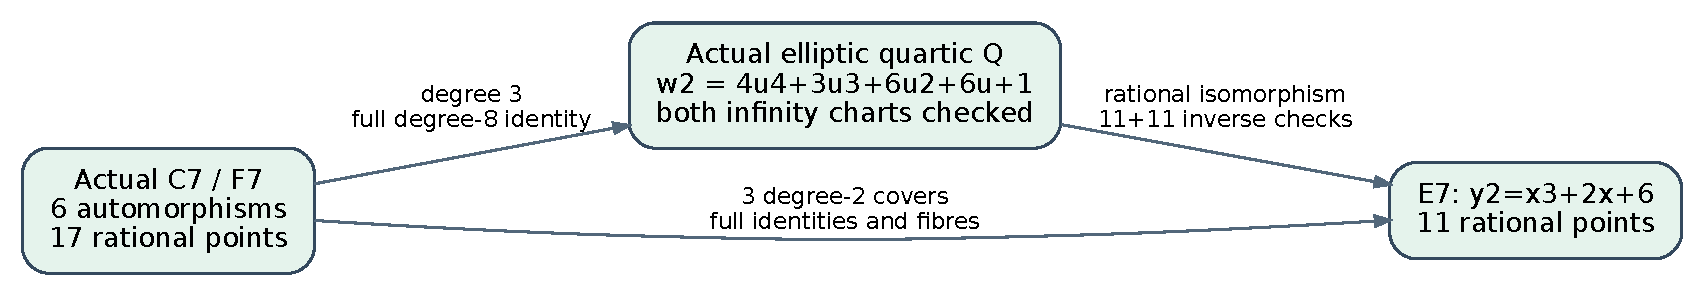
\includegraphics[width=\linewidth,height=53mm,keepaspectratio]{maps.pdf}
\end{center}

\textbf{Complete rational automorphism classification.}
Every automorphism sends a fixed projective four-frame to one of 57120
ordered distinct image frames. All decisions are retained in a complete
two-bit codec: 20304 non-general frames, 36810 point-set rejections, zero
coefficient rejections, six accepted. Each accepted matrix has all 15
quartic coefficients and its actual 17-point permutation checked.
The group orders are $1,2,3,2,2,3$, with full multiplication/inverse tables.
This is F7 completeness via the canonical embedding, not an extension census.

\textbf{The three degree-two covers.}
For the deck quotient, away from $Y=0$,
\[
 x_E=X/Y,\qquad y_E=(Z^2+6X^2+3XY+Y^2)/Y^2.
\]
The target is $E_7:y_E^2=x_E^3+2x_E+6$. At $Y=0$ the image is O.
Conjugating by actual automorphisms gives all three deck-conjugate covers.
Each has eight double fibres, one singleton and two empty rational fibres,
with all 17 images, involution invariance and full coefficient identities.
The two original infinity preimages $[1:0:\pm1]$ are retained.

\textbf{An actual degree-three quotient.}
For the first order-three map, the coordinate change
\[
 [X:Y:Z]=[x+y+z:5x:y-z]
\]
gives $x^4+3x^2yz+2xy^3+2xz^3+2y^2z^2=0$. Put
\[
 u=yz/x^2,\quad v=y^3/x^3,\quad w=4v+1+3u+2u^2.
\]
The quotient is the genuine elliptic quartic
\[
 Q:\quad w^2=4u^4+3u^3+6u^2+6u+1.
\]
Both fixed points at $x=0$ map explicitly to the two quartic infinities,
with signs $-2$ and $+2$. A full homogeneous degree-eight identity and
actual altered-constant/restoration controls pass.

Source \texttt{3916f563}; full result \texttt{62daac1e}; unsigned data
\texttt{PCC-20261123-941363}. [pcc:unverified]
\newpage
{\Large\bfseries Elliptic conversion, controls and remaining bridge}\par

\textbf{Explicit conversion and its exceptional points.}
The exact generic quartic conversion gives generalized Weierstrass
coefficients $(a_1,a_2,a_3,a_4)=(5,4,6,2)$, short model $(a,b)=(4,6)$,
and scaling three to E7. Equivalently, on the finite chart set
\[
 \delta=w+2u^2+6u+3,\qquad
 x_E=\delta+1,\quad y_E=(5u+4)\delta+4.
\]
The positive infinity maps to O, the negative infinity to $(1,3)$,
and the finite zero-delta exception is $(u,w)=(3,3)$ mapping to $(1,4)$.
The native generic formulas check the full polynomial identity modulo
$w^2-f(u)$ and all eleven quartic points and eleven E7 points in both
directions. An actual target constant mutation fails, and restoration passes.
No group structure is fabricated on the quartic points.

\textbf{Working fibres and group controls.}
The degree-three map has five triple fibres, two ramified singleton fibres
and four empty fibres on E7(F7), with all 17 source images and order-three
orbit invariance checked. The E7 group law has 121 addition pairs,
1331 associative triples and eleven order/scalar controls. Identity/deck
automorphisms pass; a real singular matrix and a wrong diagonal map fail.
Source points are read from the frozen prior output; no old whole-curve or
integral-H census is replayed.

\textbf{A concrete next Jacobian step.}
Each genuine degree-two/three cover induces actual Jacobian pushforward and
pullback correspondences. The standard composition is multiplication by
the cover degree, so pullback is injective on 11-torsion. That is a written
functorial argument, not a full native genus-three divisor group or generic
Mathlib theorem. The next construction is to combine the elliptic covers
into an odd-degree correspondence basis, then transport the nontrivial
CM19 four-map with actual divisor, polarization and target checks.

\textbf{Cost standing.}
The original subgroup has order about p, even though the Jacobian has size
about $p^3$. The published quartic $\widetilde O(p)$ bound alone gives no
ECDLP exponent gain over rho's $O(\sqrt\ell)$ reference. Full conversion,
setup, maps, solve, replay and memory costs still need a separately promising
mechanism. No benchmark, cryptographic solve or computational advantage is
claimed here.

\textbf{Execution, custody and failures.}
All seven strict B phases exit zero; guards unchanged. Rust1.99.1,
warnings denied, overflow/debug assertions, one worker, 2GiB/120s per phase.
All 22 complete locked inputs were read back before execution and all 44
result-commit files afterward.

Full stdout is 38330 bytes, SHA256
\texttt{343d44f2\ldots a158e443}, including every frame decision.
All 38 small original B records are public, and the first 35999-byte
formatting negative remains immutable. The original 4799552-byte ELF is
temporary custody-pending. The existing artifact policy passes for this
unit; parent5019's separate 82KB raw migration is still required.

\href{https://github.com/isogeny-labs/crypto/tree/3916f563ce5717f50ee1716ac10a9c979e5f656c/research/chained_cm19_curve_maps_20261123}{Frozen source/protocol}
and
\href{https://github.com/isogeny-labs/crypto/tree/62daac1e0c57cf04009fb57952dd6975339facd5/research/chained_cm19_curve_maps_20261123}{complete native results}.
Canonical-model and CM19 context: Ritzenthaler2010, DOI
\href{https://doi.org/10.1112/S1461157009000576}{10.1112/S1461157009000576}.
KB/Conductor unavailable; no novelty clearance. Generic formal proofs,
actual divisor/S maps, independent replay, approved custody and all
paid/vault/CI/merge requirements remain. [pcc:unverified]
\end{document}
